\chapter{Exploration of energy efficient memory organisations for dynamic multimedia applications using system scenarios}

\begin{center}
Iason Filippopoulos, Francky Catthoor and Per Gunnar Kjeldsberg
\\
Design Automation for Embedded Systems
\\
Springer
\\
2014
\end{center}
\afterpage{\null\newpage}
\newpage

\vspace*{\fill}
%\addcontentsline{toc}{section}{Abstract}
\section*{\hspace*{\fill} Abstract \hspace*{\fill}}
We propose a memory-aware system scenario approach that exploits variations in memory needs during the lifetime of an application in order to optimize energy usage. 
Different system scenarios capture the application's different resource requirements that change dynamically at run-time. 
In addition to computational resources, the many possible memory platform configurations and data-to-memory assignments are important system scenario parameters. 
In this work we focus on clustering of different memory requirements into groups and presenting the system scenario generation in detail.
The clustering is a non-trivial problem due to the many different memory requirements, which leads to a very large exploration space.
An extended memory model is used as a practical enabler, in order to evaluate the methodology. 
The memory models include existing state-of-the-art memories, available from industry and academia, and we show how they are employed during the system design exploration phase. 
Both commercial SRAM and standard cell based memory models are explored in this study. 
The effectiveness of the proposed methodology is demonstrated and tested using a large set of multimedia benchmarks published in the Polybench, Mibench and Mediabench suites,
representative for the domain of multimedia applications.
Reduction in energy consumption in the memory subsystem ranges from 35\% to 55\% for the chosen set of benchmarks.
\vspace*{\fill}
\afterpage{\null\newpage}
\newpage

\section{Introduction}
\label{sec:introductionC}

Modern embedded systems are becoming more and more powerful as the semiconductor processing techniques keep increasing the number of transistors on a single chip. 
Consequently, demanding applications, e.g., in the signal processing and multimedia domains, can be executed on these devices \cite{narasinga}. 
On the other hand, the desired performance has to be delivered with minimum power consumption due to the limited energy available in mobile devices \cite{tcm}. 
System scenario methodologies propose the use of different platform configurations in order to exploit run-time variations in computational and memory needs often seen in such applications \cite{tcm}.

Platform reconfiguration is performed through tuning of different system parameters, also called system knobs. 
For the memory-aware system scenario methodology, a platform can be reconfigured through a number of potential knobs, each resulting in different performance and power consumption in the memory subsystem. 
Foremost, modern memories support different energy states, e.g., through power gating techniques and by switching to lower power modes when not accessed. 
The second platform knob is the assignment of data to the available memory banks.
The data assignment decisions affect both the energy per access for the mapped data, the data conflicts as a result of suboptimal assignment, and the number of active banks. 
In this work a reconfigurable memory platform is constructed using detailed memory models. 
This is followed by experiments with dynamic multimedia applications in order to study the effectiveness of the methodology.

The main contribution of the current work is the development of data variable \cite{Elena2012} based system scenarios.
Previous control variable based system scenarios \cite{Gheorghita2007} are unable to handle the fine-grain behaviour of the studied multimedia applications due to their significant variation under different execution situations. 
Furthermore, compared with use case scenario approaches in which scenarios are generated based on a user's behaviour \cite{usecase}, the system scenario methodology focuses on the behaviour of the system to generate scenarios and can, therefore, fully exploit the detailed platform mapping information. 
Compared with previous work on system scenarios that has focused on the processing cores, the current work analyses the use of system scenarios on the memory organisation. 
More specifically, this work focuses on the system scenario identification phase of the methodology.
The wide range of memory requirements, the amount of different cases, and the different frequency in which each case occurs, results in a very large exploration space.
Therefore, there is a need for developing an algorithmic approach that can efficiently tackle this problem.

Another significant contribution is the extensive number of benchmark applications on which the methodology is applied.
The chosen set is representative for the domain of multimedia applications.
Furthermore, we present a categorisation of applications based on their dynamic characteristics, also applicable to the entire multimedia domain. 
For the experimental needs of this work we present for the purpose sufficiently detailed and accurate  memory models, which are used for the system design exploration.
For the multimedia domain, the current work presents a comprehensive methodology for optimising energy consumption in the memory subsystem.

This article is organized as follows. 
Section~\ref{sec:motivationC} motivates the study of optimization of the memory organisation. 
Section~\ref{sec:relatedC} surveys related work on system level memory exploration and on system scenario methodologies and compares it with the current work. 
Section~\ref{sec:methodologyC} presents the chosen methodology with main focus on the memory organisation study. 
In Section~\ref{sec:platformC} the target platform is described accompanied by a detailed description of the employed memory models, while the multimedia benchmarks and their characteristics are analysed in Section~\ref{sec:applicationsC}. 
Results of applying the described methodology to the targeted applications are shown in Section~\ref{sec:resultsC}, while conclusions are drawn in Section~\ref{sec:conclusionC}. 

\section{Motivational Example}
\label{sec:motivationC}

A large number of papers have demonstrated the importance of the memory organization to the overall system energy consumption. 
As shown in \cite{Gonzalez1996} memory contributes around 40\% to the overall power consumption in general purpose systems. 
Especially for embedded systems, the memory subsystem accounts for up to 50\% of the overall energy consumption \cite{Che09} and the cycle-accurate simulator presented in \cite{Ben99} estimates that the energy expenditures in the memory subsystem range from 35\% up to 65\% for different architectures. 
The breakdown of power consumption for a recently implemented embedded system presented in \cite{Hul11} shows that the memory subsystem consumes more than 40\% of the leakage power on the platform. 
According to \cite{tcm}, conventional allocation and assignment of data done by regular compilers is suboptimal. 
Performance loss is caused by stalls for fetching data and data conflicts for different tasks, due to the limited size of memory and the competition between tasks. 

\begin{algorithm}
\caption{Motivational example of dynamic memory usage}
 \label{alg:motivation}
 \begin{algorithmic}[1]
	\WHILE{$image \ne EndOfDatabase$}
		\STATE $height \gets height(image)$
		\STATE $width \gets width(image)$
		\STATE $store(image[height][width])$
			\FOR{$i = 0 \to height$} 
				\FOR{$j = 0 \to width$} 
					\STATE $array[i][j] \gets func1(image[i][j])$
				\ENDFOR
			\ENDFOR
		\STATE $image \gets new.image$	
	\ENDWHILE
 \end{algorithmic}
\end{algorithm}

In addition, modern applications exhibit more and more dynamic behaviour, which is reflected also in fluctuating memory requirements \cite{tcm}. 
Techniques have been developed in order to estimate the memory size requirements of applications in a systematic way \cite{Ang13}. 
The significant contribution that the memory subsystem has to the overall energy consumption of a system and the dynamic nature of many applications offer a strong motivation for the study and optimization of the memory organisation in modern embedded devices.

To illustrate the sub-optimal conventional allocation and assignment of data, the simple example of Alg.~\ref{alg:motivation} is used. 
The kernel code of an image processing application continuously reads a sequence of images, saves each image in memory and performs function \textit{func1} on each pixel of the image. 
Arrays are typically used for storing the intermediate calculations in image processing applications, exemplified with the \textit{array} variable in the motivation example. 
The memory size used for the storage of each initial \textit{image} and the computed \textit{array} are determined by the dimensions of the input image and can be different for a series of input images. 
In a conventional assignment the highest values of \textit{height} and \textit{width} are identified and a static compiling results in allocation of the worst-case area for the \textit{array} variable. 
However, only a part of the allocated space is accessed during processing of smaller images. 

Assume for instance that we have two different image sizes, ImgA with L=H=1 and ImgB with L=H=2. 
That is, the size of ImgB is 4 $\times$ ImgA. 
Each pixel in each image is accessed once giving rise to N accesses to each ImgA and 4 $\times$ N accesses to each ImgB. 
Furthermore, in the input stream of images there are four times as many ImgA as ImgB. 
In our pool of alternative memories we have three memories with Size1 = ImgA, Size2  = 3 $\times$ ImgA, and Size 3 = 4 $\times$ ImgA (i.e., the size of ImgB). 
The energy cost of accessing a Size1 memory is 1E, while the average leakage energy in the time between the start of two accesses is 0.3E. 
The corresponding access/leakage numbers for Size2 and Size3 memories are 1.3E/0.9E and 1.5E/1.2E, respectively. 
The numbers reflects the fact that as a first order approximation access energy increases sub linearly with increased memory size, while leakage increases linearly with memory size. 
The total energy (access + leakage) during computations on four ImgA and one ImgB using only one memory of Size3 is:
\begin{align*}
4 \times N \times 1.5E + 4 \times N \times 1.5E + 8 \times N \times 1.2E = 21.6NE
\end{align*}
The same calculation using one memory of Size1 and one of Size2, in total the size of ImgB, is: 
\begin{align*}
& 4 \times N \times 1.0E + 1 \times N \times 1.0E + 3 \times N \times 1.3E \\
& + 4 \times N \times 0.3E + 4 \times N \times (0.3E + 0.9E) =  14.9NE
\end{align*}
giving a reduction in energy consumption of 31\%. 
These calculations are done with simplified assumptions regarding input data and memory models. 
The results in Section~\ref{sec:resultsC} show even larger gain with realistic dynamic applications, memory models and data.

\section{Related Work and Contribution Discussion}
\label{sec:relatedC}

%Many papers have focused on memory related optimisations, also in the presence of a partitioned and distributed memory organisation with memory blocks of different sizes. 
%In \cite{Ben00b} authors present a methodology for automatic memory hierarchy generation that exploits memory access locality, while in \cite{Ben00c} they propose an algorithm for the automatic partitioning of on-chip SRAM in multiple banks. 
The memory allocation problem has been studied before. 
However, we extend state of the art by proposing a more generic approach, which is also suitable for applications with input driven dynamic behaviour. 
The authors in \cite{Ben00b} present a methodology to generate a static application-specific memory hierarchy. 
Later, they extend their work in \cite{Ben00c} to a reconfigurable platform with multiple memory banks. 
However, our work differentiates by proposing a more generic and application agnostic methodology and employing the use of system scenarios, in order to efficiently handle a wider range of dynamic application characteristics. 

Several techniques for designing energy efficient memory architectures for embedded systems are presented in \cite{Mac02}. 
The current work differentiates by employing a platform that is reconfigurable at run-time. 
In \cite{Pgk01} a large number of data and memory optimisation techniques, that could be dependent or independent of a target platform, are discussed. 
Again, reconfigurable platforms are not considered.

Energy-aware assignment of data to memory banks for several task-sets based on the MediaBench suit of benchmarks is presented in \cite{Mar03}. 
Low energy multimedia applications are discussed also in \cite{Chu02} with focus on processing rather than the memory platform. 
Furthermore, both \cite{Mar03} and \cite{Chu02} base their analysis on use case situations and do not incorporate sufficient support for very dynamically behaving application codes. 
System scenarios alleviate this bottleneck and enable handling of such dynamic behaviour. 
In addition, the current work explores the assignment of data to the memory and the effect of different assignment decisions on the overall energy consumption.

The authors in \cite{abraham1999automatic}, \cite{jacob1996analytical} and \cite{li1999hardware} present methodologies for designing memory hierarchies.
Design methods with main focus on the traffic and latencies in the memory architecture are presented in \cite{chen1999loop}, \cite{grun2000mist}, \cite{jantsch1994hardware} and \cite{passes1995multi}.
Improving memory energy efficiency based on a study of access patterns is discussed in \cite{kandemir2001improving}.
Application specific memory design is a research topic in \cite{schmit1997synthesis}, while memory design for multimedia applications is presented in \cite{oshima1997high}.
The current work differentiates by introducing the concept of system scenarios that supports the dynamic handling of application's requirements, although the data mapping is static inside each scenario. 

An overview of work on system scenario methodologies and their application are presented in \cite{Gheorghita2007}. 
In \cite{Fil12} extensions towards a memory-aware system scenario methodology are presented and demonstrated using theoretical memory models and two target applications. 
This work is an extension both in complexity and accuracy of the considered memory library and on the number of target applications. 

Furthermore, the majority of the published work focus on control variables for system scenario prediction and selection. 
Control variables can take a relatively small set of different values and thus can be fully explored. However, the use of data variables \cite{Elena2010} is required by many dynamic systems including the majority of multimedia applications. 
The range of possible values for data variables is wider and makes full exploration impossible. 

Authors in \cite{Pal06} present a technique to optimise memory accesses for input data dependent applications by duplicating and optimising the code for different execution paths of a control flow graph (CFG). 
One path or a group of paths in a CFG form a scenario and its memory accesses are optimised using global loop transformations (GLT). 
Apart from if-statement evaluations that define different execution paths, they extend their technique to include while loops with variable trip count in \cite{Pal06b}. 
A heuristic to perform efficient grouping of execution paths for scenario creation is analysed in \cite{Pal07}. 
Our work extends the existing solutions towards exploiting the presence of a distributed memory organisation with reconfiguration possibilities.

Reconfigurable hardware for embedded systems, including the memory architecture, is a topic of active research. 
An extensive overview of current approaches is found in \cite{Garcia}. 
The approach presented in this paper differentiates by focusing on the data-to-memory assignment aspects in the presence of a platform with dynamically configurable memory blocks. 
Moreover, many methods for source code transformations, and especially loop transformations, have been proposed in the memory management context. 
These methods are fully complementary to our focus on data-to-memory assignment and should be performed prior to our step. 

\section{Data Variable Based Memory-Aware System Scenario Methodology}
\label{sec:methodologyC}

The memory-aware system scenario methodology is based on the observation that the memory subsystem requirements at run-time vary significantly due to dynamic variations of memory needs in the application code. 
Most existing design methodologies define the memory requirements as that of the most demanding task and tune the system in order to meet its needs \cite{tcm}. 
Obviously, this approach leads to unused memory area for tasks with lower memory requirements, since those tasks could meet their needs using fewer resources and consequently consuming less energy. 
Another source of energy waste in the memory system is caused by data conflicts due to misplaced data. 
Replacement of old data and fetching of new data is both time and energy consuming and should therefore be avoided. 
Handling of data conflicts is also part of a memory-aware system scenario methodology.

Designing with system scenarios is workload adaptive and offers different configurations of the platform and the freedom of switching to the most efficient scenario at run-time. 
A system scenario is a configuration of the system that combines similar run-time situations (RTSs). 
An RTS consists of a running instance of a task and its corresponding cost (e.g., energy consumption) and one complete run of the application on the target platform represents a sequence of RTSs \cite{Elena2010}. 
The system is configured to meet the cost requirements of an RTS by choosing the appropriate system scenario, which is the one that satisfies the requirements using minimal power. 
In the following subsections, the different steps of the memory-aware system scenario methodology are outlined. 

The system scenario methodology follows a two stage exploration, namely design-time and run-time stages, as described in \cite{Gheorghita2007}. 
This splitting is also employed in the memory-aware extension of the methodology. 
The two stage exploration is chosen because it reduces run-time overhead while preserving an important degree of freedom for run-time configuration \cite{tcm}. 
The application is analysed at design-time and different execution paths causing variations in memory demands are identified. 
This procedure, which is time consuming and as a result can be performed only during the design phase, will result in a grey-box model representation of the application. 
The grey-box model hides all static and deterministic parts of the application, instead only providing their related memory costs to the system designer.
Parts of the application code that are non-deterministic in terms of memory usage are directly available to the system designer \cite{graybox}. 


\subsection{Design-time Profiling Based on Data Variables}

\begin{figure}
\centering
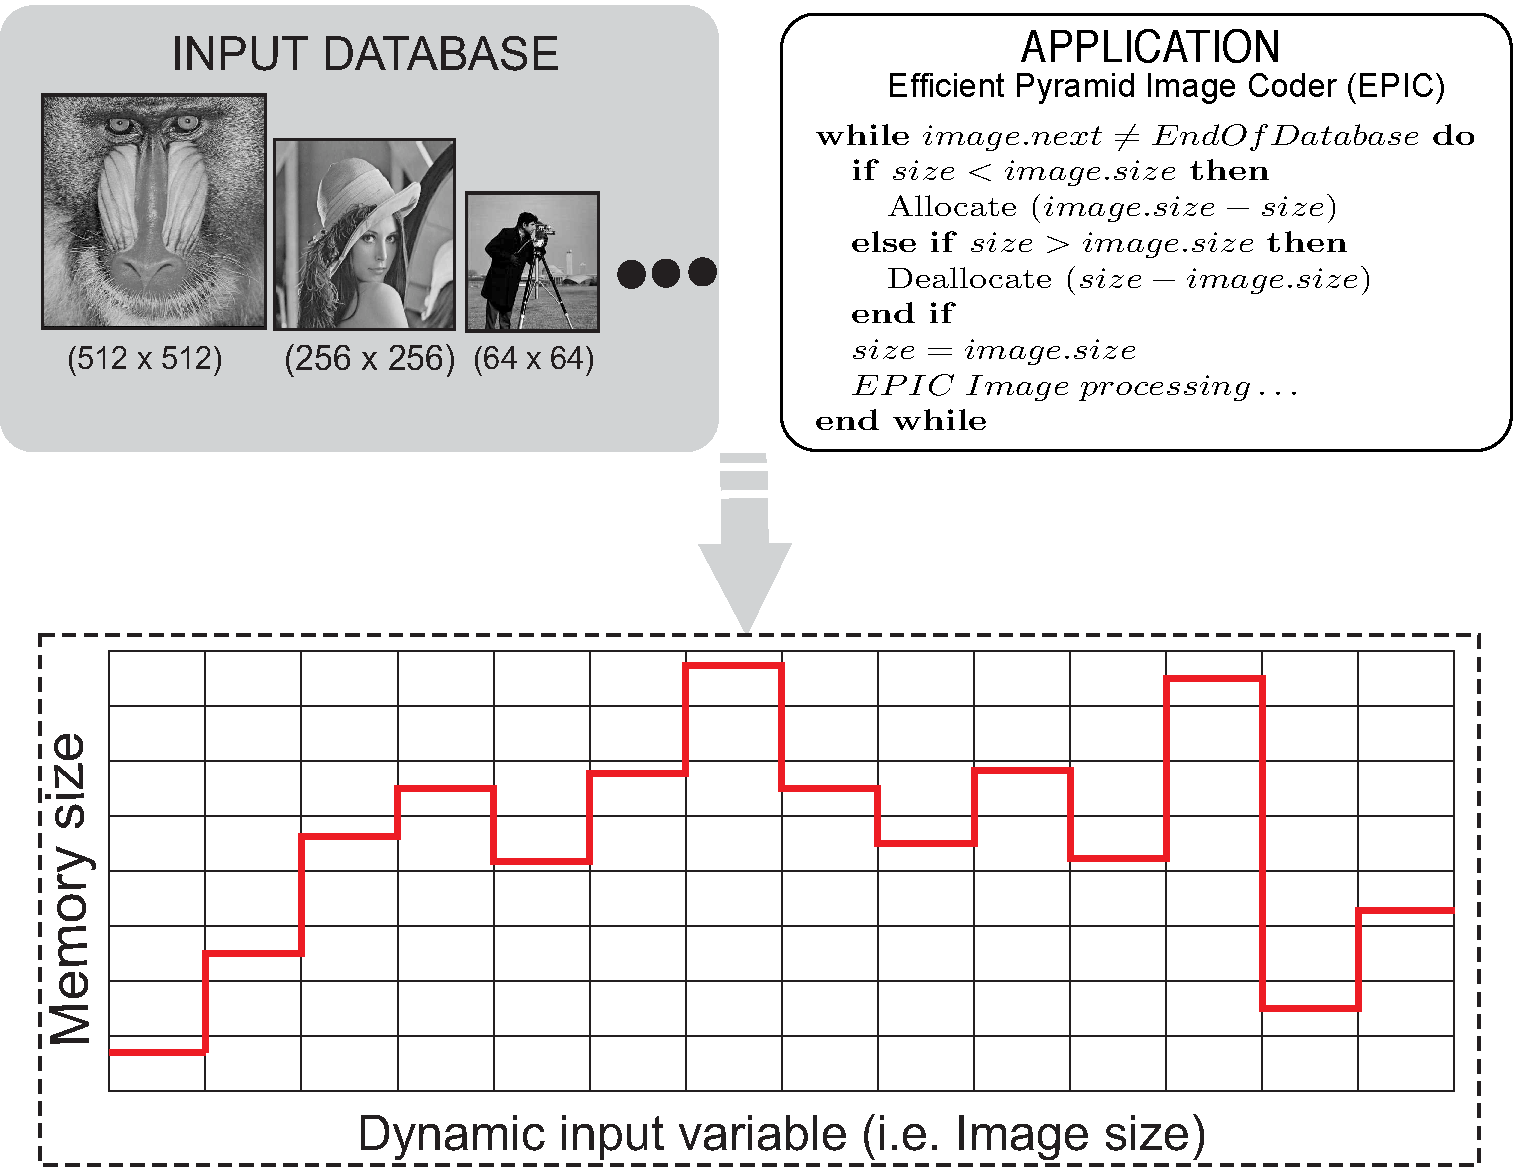
\includegraphics[width=0.75\textwidth]{C/profiling2.pdf}
\caption{Profiling results based on application code and input data}
\label{fig:profilingC}
\end{figure}

Application profiling is performed at design-time for a wide range of inputs. 
The analysis focuses on the allocated memory size during execution and on access pattern variations. 
Techniques described in \cite{Ang13b} are, e.g., used in order to extract the access scheme through analysis of array iteration spaces.  

The profiling stage is depicted in Fig.~\ref{fig:profilingC} and consists of running the application code with suitable input data often found in a database, in order to produce profiling results. 
The results shown here are limited for demonstrational purposes. 
A real application would have thousands or millions of profiling samples. 
The profiling reveals parts of the application code with high memory activity and with varying memory access intensity, which possibly depends on input data variables. 
Because of this behaviour, a static study of the application code alone is insufficient since the target applications for this methodology have non-deterministic behaviour that is driven by input.

Profiling results provided to the designer include complete information about allocated memory size values together with the number of occurrences and duration for each of these memory size values. 
Moreover, correlation between input data variable values and the resulting memory behaviour can possibly be observed. This information is useful for the clustering step that follows. 
Profiling also reveals the worst case memory usage for a given set of inputs. 
The memory usage is measured using techniques presented in \cite{Ang13b}, in which authors compute the minimum amount of memory resources required to store the elements of an application. 

In Fig.~\ref{fig:profilingC} the profiled applications are two image related multimedia benchmarks and the input database should consist of a variety of images. 
The memory requirements in each case are driven by the current input image size, which is classified as a data variable due to the wide range of its possible values. 
Depending on the application the whole image or a region of interest is processed. 
Other applications have other input variables deciding the memory requirement dynamism, e.g., the channel SNR level in the case of an encoding/decoding application.

The input data used for profiling are generated based on realistic assumptions for each of the chosen benchmarks. 
Each application is studied and based on its functionality, a range of rational inputs are developed. 
In addition, example inputs are available for most of the studied benchmark applications. 
The choice of common and open-source benchmarks provides us the opportunity to find inputs publicly available. 
Based on the collected information, we define the range of realistic inputs and we generate a random set on inputs within these limits. 
For example, the bibliography provides information for the real SNR levels and the constraint length of the Viterbi encoder for each level, in order to achieve a  successful communication. 
For profiling, we generate randomly a set of SNR levels that cover this whole range. 
Similar technique is used for the applications that use an image as an input. 
First, we explore the sizes of images commonly used to define the minimum and the maximum size and then we randomly generate a set of image sizes within the size limits. 
For the random generation of inputs, we assume the same probability for each situation, because there is no information available regarding the frequency of each input. 
As a result the frequency of each input is random. 

\subsection{Design-time System Scenario Identification Based on Data Variables}

\begin{figure}
\centering
\includegraphics[width=0.75\textwidth]{C/1Dclustering.pdf}
\caption{Clustering of profiling results into three (a) or five (b) system scenarios}
\label{fig:clusteringC}
\end{figure}

The next step is the clustering of the profiled memory sizes into groups with similar characteristics. 
This is referred to as system scenario identification. 
Clustering is necessary, because it will be extremely costly to have a different scenario for every possible size, due to the number of memories needed. 
Clustering neighbouring RTSs is a rational choice, because two instances with similar memory needs have similar energy consumption. 

In Fig.~\ref{fig:clusteringC} the clustering of the previously profiled information is presented. 
The clustering of RTSs is based both on their distance on the memory size axis and the frequency of their occurrence. 
Consequently, the memory size is split unevenly with more frequent RTSs having a shorter memory size range. 
In the case of a clustering to three system scenarios the space is divided in the three differently coloured hashed areas depicted in Fig.~\ref{fig:clusteringC}(a). 
Due to the higher frequency of RTSs in the yellow hashed area, that system scenario has a shorter range compared with its neighbouring scenarios. 
Such clustering is better than an even splitting because the energy cost of each system scenario is defined by the upper size limit, as each scenario should support all RTSs within its range. 
Consequently the overhead for the RTSs in the yellow area is lower compared to the overhead in the two other areas.

The same principle applies also when the number of system scenarios is increased to five, as depicted in Fig.~\ref{fig:clusteringC}(b). 
The frequency sensitive clustering results in two short system scenarios that contain four RTSs each and three wider system scenarios with lower numbers of RTSs. 
The number of system scenarios should be limited mainly due to two factors. 
First, implementation of a high number of system scenarios in a memory platform is more difficult and complex. 
Second, the switching between the different scenarios involves an energy penalty that could become significant when the switching takes place frequently.

The memory size and the frequency of each RTS are not the only two parameters that should be taken into consideration during the system scenario identification. 
The memory size of each RTS results in a different energy cost depending on the way it is mapped into memory. 
The impact of the different assignment possibilities is included into the clustering by introduction of energy as a cost metric. 
The energy cost for each RTS is calculated using a reference platform with one to N
memory banks. 
Increasing the number of memory banks results in lower energy per access since the most accessed elements can be assigned to smaller and more energy efficient banks. Unused banks can be switched off.

In the system scenario methodology, Pareto curves are used to capture alternative system configurations within a scenario \cite{tcm}. 
In our work, a Pareto space is used for clustering that also includes the energy cost metric. 
For each RTS all different assignment options on alternative platform configurations are studied. 
Memory platform knobs are different sets of memory banks that are turned on and off.
A Pareto curve is constructed for each RTS that contains the optimal assignment for each platform configuration. 
Hence, suboptimal assignments and assignments that result in conflicts are not included in the Pareto curve. 
In Fig.~\ref{fig:paretoC} four Pareto curves, each corresponding to a different RTS, are shown together with energy cost levels corresponding to different platform configuration and data-to-memory assignment decisions. 
Three non-optimal mappings are also shown in Fig.~\ref{fig:paretoC} for illustration. 
They are not part of the Pareto curve and consequently not included in the generation of scenarios. 
Pareto curves are clustered into three different system scenarios based again both on their memory size differences and frequency of occurrence. 
Clustering of RTSs using Pareto curves is more accurate compared to the clustering depicted in Fig.~\ref{fig:clusteringC}, as it includes data-to-memory assignment options in the exploration. 

\begin{figure}
\centering
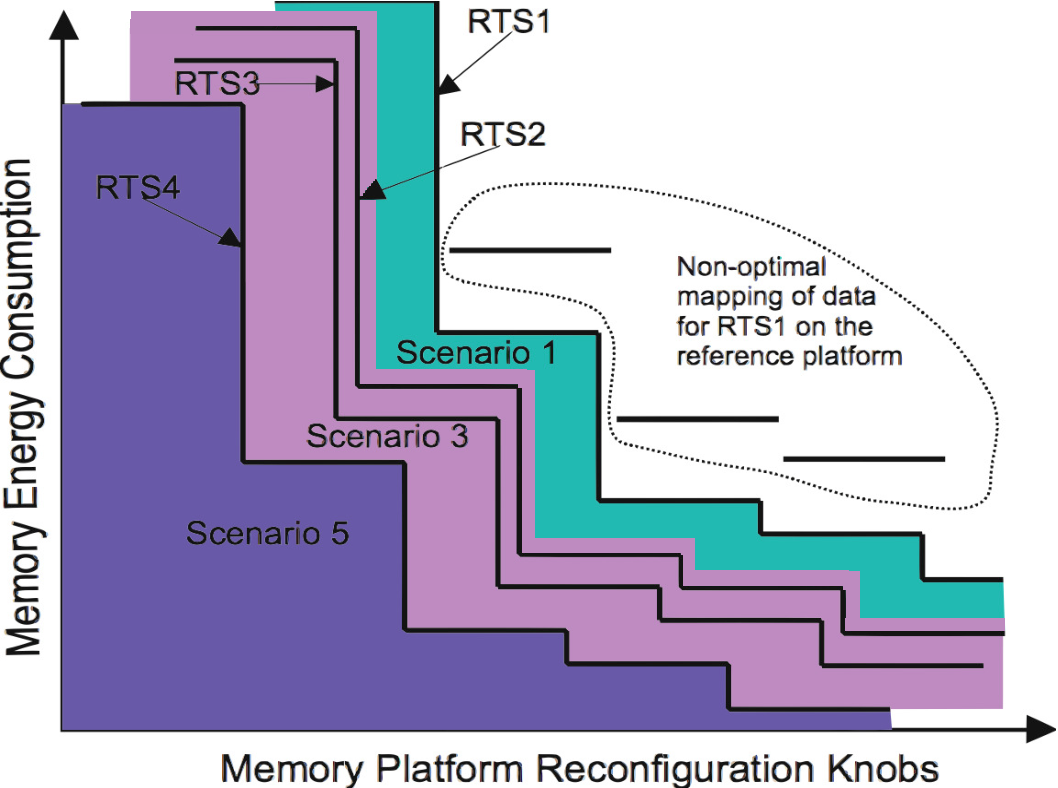
\includegraphics[width=0.75\textwidth]{C/2D.pdf}
\caption{Clustering of Pareto curves}
\label{fig:paretoC}
\end{figure}

The system scenario identification step includes the selection of the data variables that determine the active system scenario. 
This can be achieved by careful study of the application code, combined with the application's data input.
The variable selection is done before clustering of RTSs into scenarios.
For the choice of identification variables, there is a trade-off between the complexity and the accuracy of the scenario detection step.
On one hand, if the identification is done using a group of complex variables and their correlation, there is a number of calculations needed in order to predict the active scenario. 
On the other hand, if the value of a single variable is monitored for scenario identification, the scenario detection is straightforward.
Obviously, the accuracy of the scenario detection is higher on the first case, while the computational needs for scenario detection are lower on the second case.
In other words, the more accurate scenario detection, the more resources are used by the run-time manager for detection.
In our case the grey-box model reveals only the code parts that will influence memory usage, so that data variables deciding memory space changes can be identified. 
An example of this is a non static variable that influences the number of iterations for a loop that performs one memory allocation at each iteration. 
In the depicted example the system scenario detection data variable is the input image height and width values. 
Moreover, the designer should look for a correlation between input values and the corresponding cost. 
This information will be useful in the following steps of the methodology \cite{tcm}.

\subsection{Run-time System Scenario Detection and Switching Based on Data Variables}

Switching decisions are taken at run-time by the run-time manager. 
In this work, we use a simple and straightforward switching approach.
Memory models provide the necessary information for the switching decision, namely the energy and the time penalty for switching between stages.
The switching step consists of all platform configuration decisions that can be made at run-time, e.g., frequency/voltage scaling, changing the power mode of memory units, including turning them off, and reassignment of data to memory units. 
Switching takes place when the switching cost is lower than the energy gains achieved by switching. 

In more detail, the switching mechanism implemented by the run-time manager includes the following actions: 
\begin{enumerate}
\item Calculation of the energy consumption by processing the next input on the currently active scenario (E1).
\item Calculation of the energy consumption by processing the next input on its most energy efficient scenario (E2).
\item Calculation of the energy penalty for switching the needed memory banks to the configuration of the most efficient scenario (E3).
\item Evaluation of the expression: E1 \textgreater  E2 + E3. If the energy cost of the current configuration (E1) is greater than the combined cost of the new configuration and the required switching (E2 + E3), then the decision is to switch. Otherwise, the switching decision is negative and the system stays on the currently running configuration
\item Switching of the platform to its new configuration. The memory banks switch to the appropriate state, which is defined by the chosen scenario. 
\end{enumerate}
% the run-time manager compares the memory energy consumption of executing the next task in the current active system scenario with the energy consumption of execution with the optimal system scenario. 
%If the difference is greater than the switching cost, then scenario switching is performed \cite{tcm}. 
Switching costs are defined by the platform and include all memory energy penalties for run-time reconfigurations of the platform, e.g., extra energy needed to change state of a memory unit.

The run-time manager is minimal, resulting in a very small overhead, and is complementary to an operating system (OS), if such is available on the platform. 
In the presence of an embedded OS, the OS needs to start the runtime manager and grant it access to system reconfiguration calls. 
In both cases, when the run-time manager is active, it performs a few simple steps with minimal system performance overhead. 
In more detail, the run-time manages checks the current state of the monitored identification variable(s), determine the next scenario based on this value and decides whether switching should be performed. 
The corresponding scenario for a given value of the identification variable is a simple look-up, because all the analysis has been performed at design-time. 
The hardware configuration for the active scenario is also explored at design-time and the run-time manager is aware of the required changes. 
In our approach no need is present for modifications of the application code.
Instead, we add the above mentioned changes in the middleware layer. 
That has the additional advantage that the run-time manager is reusable across several tasks/processes running at the application layer on top of this shared middleware. 
The application data are stored and accessed the same way at the application level. 
The difference with the proposed approach is the size and the state of the memory bank that the data are stored in. 
The application is unaware of the exact way the data is stored and accessed and the methodology ensures that the accessed addresses in the application code always corresponds to an active bank.

\begin{figure}
\centering
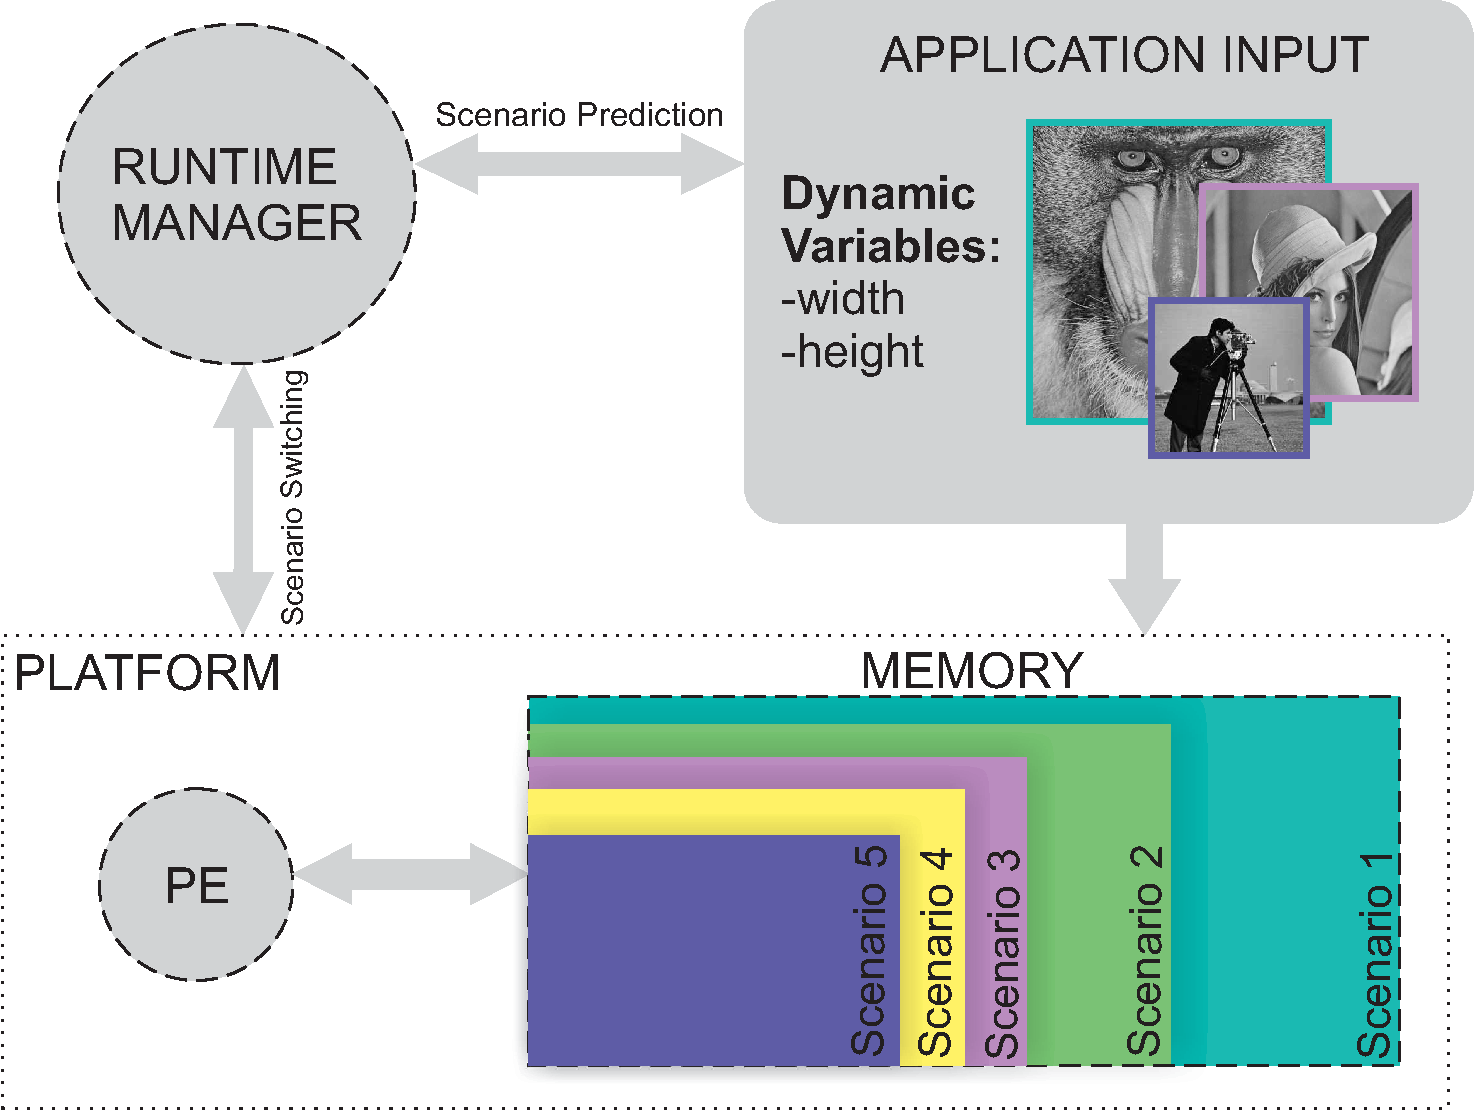
\includegraphics[width=0.75\textwidth]{C/switching.pdf}
\caption{Run-time system scenario detection and switching based on the current input}
\label{fig:runtimeC}
\end{figure}

In Fig.~\ref{fig:runtimeC} an example of the run-time phase of the methodology is depicted. 
The run-time manager identifies the size of the image that will be processed and reconfigures the memory subsystem on the platform, if needed, by increasing or decreasing the available memory size. 
The reconfiguration options are effected by platform hardware limitations. 
The image size is in this case the data variable monitored in order to detect the system scenario and the need for switching.

\section{Target Platform and Energy Models}
\label{sec:platformC}

Selection of target platform is an important aspect of the memory-aware system scenario methodology. 
The key feature needed in the platform architecture is the ability to efficiently support different memory sizes that correspond to the system scenarios generated by the methodology. 
Execution of different system scenarios then leads to different energy costs, as each configuration of the platform results in a specific memory energy consumption. 
The dynamic memory platform is achieved by organising the memory area in a varying number of banks that can be switched between different energy states. 

\subsection{Target Memory Platform Architecture}

In this work, a clustered memory organisation with up to five memory banks of varying sizes is explored. 
The limitation in the number of memory banks is necessary in order to keep the interconnection cost between the processing element (PE) and the memories constant through exploration of different architectures. 

For more complex architectures the interconnection cost should be considered and analysed separately for accurate results. 
Although power gating can be applied to the bus when only a part of a longer bus is needed, an accurate model of the memory wrapper and interconnection must developed, which is beyond the scope of the current work. 

\begin{figure}
\centering
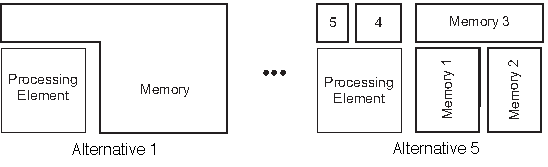
\includegraphics[width=0.75\textwidth]{C/platform.pdf}
\caption{Alternative memory platforms with varying number of banks}
\label{fig:platformC}
\end{figure}

%Minor revision comment 2
Some examples of alternative memory platforms that can be used for exploration is shown in Fig.~\ref{fig:platformC}. 
Point-to-point connections with negligible interconnect costs between elements are assumed for up to five memory banks. 
The decision to use memory banks with varying sizes on the clustered memory organization increases the reconfiguration options and consequently the potential energy gains. 
In general, smaller memories are more energy efficient compared to larger memories banks. 
However, in some cases large memory banks are needed in order to fit the application data without the need for too many small memories causing complex interconnects. 
The goal is to use the most energy efficient banks to store the most frequently used data. 
The calculations needed for enabling the minimum number of banks is simple, given the application requirements for the current input and the sizes of the five memory banks.

\subsection{Models of Different Memory Types}
The dynamic memory organisation is constructed using commercially available SRAM memory models (MM).
For those models delay and energy numbers are derived from a commercial memory compiler.
In addition, experimental standard cell-based memories (SCMEM) \cite{Mei11}  are  considered for smaller memories due to their energy and area efficiency for reasonably small storage capacities, as argued in \cite{Mei10}. 
The standard cell-based memories are synthesized using Cadence RTL compiler for TSMC 40nm standard library. 
Afterwords, power simulations on the synthesized design are carried out using Synopsys PrimeTime, in order to obtain energy numbers.
Both MMs and SCMEMs can operate under a wide range of supply voltages, thus support different operating modes that provide an important exploration space.
\begin{itemize}
\item Active mode: The normal operation mode, in which the memory can be accessed at the maximum supported speed. The supply voltage is 1.1V. 
The dynamic and leakage power are higher compared to the other modes.
Only on active mode the data are accessible without time penalties, in contrast to light and deep sleep modes.
In this work all the memory accesses are performed in active mode. 
\item Light sleep mode: The supply voltage in this mode is lower than active with values around 0.7V. 
The access time of the memory is significantly higher than the access time in active mode. 
Switching to active mode can be performed with a negligible energy penalty and a small time penalty of a few clock cycles (less than 10). 
Data is retained.  
\item Deep sleep mode: The supply voltage is set to the lowest possible value that can be used without loss of data. 
This voltage threshold is expected to be lower for SCMEMs than MM models and can be as low as 0.3V. 
The number of clock cycles needed for switching to active mode is higher compared to sleep mode, typically in the range of 20 to 50 clock cycles depending on the clock speed. 
Consequently, the speed of the PE and the real-time constrains of the applications has to be taken into consideration when choosing light or deep sleep mode at a specific time.  
\item Shut down mode: Power-gating techniques are used to achieve near zero leakage power. 
Stored data is lost. 
The switch to active mode requires substantially more energy and time. 
However, switching unused memories to this mode, providing that their data are not needed in the future, results in substantial energy savings.
\end{itemize}  

%Minor revision comment 1
The exploration includes memories with 4 energy modes in contrast to a more conservative approach that assumes only on and off states. 
This is in line with is modern energy efficient memories that tend to support an increasing number of energy modes as a feature. 
The methodology is still applicable to a memory organization that supports only two modes, but the intention of this work is to explore the state of the art memory technologies.
The policy for switching between the modes depends on the reuse of the stored data, which  depends on the nature of the target application.
The switching policy is determined by examining the following condition for the stored data in a memory bank:
\begin{itemize}
\item If the data is currently under processing, then the only acceptable mode is the active mode.
\item If the data is not accessed, but will be needed in the near future, then the light or deep sleep mode should be chosen.
\item If the processing of the data is completed and the application is not accessing them again, the shut-down mode is the optimal solution.
\end{itemize}

Applications that perform calculations on a set of input data to produce a result and never re-access the initial data, normally only use two modes.
The need for more energy modes arises from the fact that many applications re-access the initial data or some intermediate results.
Thus, the runtime manager chooses a sleep mode that reduces the leakage power, but retains the data for future use. 
%Another example of efficient usage of different modes is the parallel processing of data stored in multiple banks by an application.
%In this case, if there is a time consuming processing in one bank (i.e. a moving object is found in a part of the image), there is an opportunity to switch some banks in sleep mode while waiting.

The necessary energy/power information is available to the system designer and relative values for a subset of the used sizes in the current work are presented in Tab.~\ref{tab:rel1} and in Tab.~\ref{tab:rel2}. 
It shows that the choice of memory units has an important impact on the energy consumption. 
Moreover, different decisions have to be made based on the dominance of dynamic or leakage energy in a specific application. 
In the current work memory architectures with 1 to 5 memory units  of different sizes are explored and the optimal configuration is chosen. 
The methodology is in general not restricted to specific memory types or benchmarks and can handle more complex hierarchical memory architectures and applications. 
However, in this study the chosen applications have a relatively small memory space requirement limited to around 100KB, which is the case for many applications run on modern embedded systems. 

\begin{table}
	\caption{Relative dynamic energy for a range of memories with varying capacity and type}
	\label{tab:rel1}
	\begin{tabular}{|c|c|c|c|c|c|}
		\hline
		\multirow{2}{*}{\textbf{Type}} & \textbf{Lines x} & \multicolumn{2}{c|}{\textbf{Dynamic Energy [J]}} & \multicolumn{2}{c|}{Switching to Active from} \\ \cline{3-4}
		& \textbf{wordlength} & Read & Write  & Deep[uJ] & Light[uJ]\\ 
		\hline 
		MM & 32 x 8 &  $ 4.18 \times 10^{-8} $ &  $ 3.24 \times 10^{-8} $ & 0.223 &  0.031 \\ 
		\hline
		MM & 32 x 16 & $  6.79 \times 10^{-8} $ &  $ 5.89 \times 10^{-8} $ & 0.223 &  0.031\\ 
		\hline
		MM & 32 x 128 & $  4.33 \times 10^{-7} $ &  $ 4.31 \times 10^{-7} $ & 1.42 & 0.168\\ 
		\hline
		MM & 256 x 128 & $  4.48 \times 10^{-7} $ &  $ 4.60 \times 10^{-7} $ & 1.70 &  0.171\\ 
		\hline
		MM & 1024 x 128 & $  5.11 \times 10^{-7} $ &  $ 5.75 \times 10^{-7} $ & 2.81 & 0.179\\ 
		\hline
		MM & 4096 x 128 & $  9.60 \times 10^{-7} $ &  $ 4.57 \times 10^{-7} $ & 9.01 & 0.457\\ 
		\hline
		SCMEM & 128 x 128 & $  2.5 \times 10^{-7} $ &  $ 0.8 \times 10^{-8} $ & 1.51 &  0.045\\ 
		\hline
		SCMEM & 1024 x 8 & $  1.7 \times 10^{-8} $ &  $ 0.6 \times 10^{-8} $ & 0.325 &  0.021\\ 
		\hline
	\end{tabular}
\end{table}

\begin{table}
	\caption{Relative static power for a range of memories with varying capacity and type}
	\label{tab:rel2}
	\begin{tabular}{|c|c|c|c|c|c|}
		\hline
		\multirow{2}{*}{\textbf{Type}} & \textbf{Lines x} & \multicolumn{4}{c|}{\textbf{Static Leakage Power per Mode[W]}} \\ \cline{3-6}
		& \textbf{wordlength} & Active & Light-sleep & Deep-sleep & Shut-down\\ 
		\hline 
		MM & 32 x 8 & 0.132 & 0.125 & 0.063 & 0.0016\\ 
		\hline
		MM & 32 x 16 & 0.134 & 0.127 & 0.064 & 0.0022\\ 
		\hline
		MM & 32 x 128 & 0.171 & 0.160 & 0.083 & 0.0112\\ 
		\hline
		MM & 256 x 128 & 0.207 & 0.184 & 0.104 & 0.0293\\ 
		\hline
		MM & 1024 x 128 & 0.349 & 0.283 & 0.189 & 0.102\\ 
		\hline
		MM & 4096 x 128 & 0.95 & 0.708 & 0.544 & 0.396\\ 
		\hline
		SCMEM & 128 x 128 & 0.083 & 0.057 & 0.027 & 0.0022\\ 
		\hline
		SCMEM & 1024 x 8 & 0.042 &
		 0.028 & 0.014 & 0.0011\\ 
		\hline
	\end{tabular}
\end{table}

\subsection{Total Energy Consumption Calculation}
Both the dynamic and the static energy consumed in the memory subsystem is included in the calculations.
The overall energy consumption for each configuration is calculated using a detailed formula, as can be seen in Eq.\ref{eq:energyC}. 
All the important transactions on the platform that contribute to the overall energy are included, in order to achieve as accurate results as possible. In particular:
\begin{itemize}
\item $N_{rd}$ is the number of read accesses
\item $E_{Read}$ is the energy per read
\item $N_{wr}$ is the number of write accesses 
\item $E_{Write}$ is the energy per write 
\item T is the execution time of the application
\item $T_{LightSleep}$, $T_{DeepSleep}$ and $T_{ShutDown}$ are the times spent in light sleep, deep sleep and shut down states respectively
\item $P_{leak_{Active}}$ is the leakage power in active mode 
\item $P_{leak_{LightSleep}}$, $P_{leak_{DeepSleep}}$ and $P_{leak_{Shutdown}}$ are the leakage power values in light sleep, deep sleep and shut down modes with different values corresponding to each mode 
\item $N_{SWLight}$, $N_{SWDeep}$ and $N_{SWShutDown}$ are the number of transitions from each retention state to active state
\item $E_{LightSleep \: to \: Active}$, $E_{DeepSleep \: to \: Active}$ and $E_{ShutDown \: to \: Active}$  are the energy penalties for each transition respectively.
\end{itemize}
\setlength{\arraycolsep}{0.0em}
\begin{eqnarray}
\label{eq:energyC}
 E &{}= {}&\sum\limits_{memories}^{all}  ( N_{rd} \times E_{Read} \nonumber\\
		&&+ N_{wr} \times E_{Write} \nonumber\\
		&&+ (T - T_{LightSleep} - T_{DeepSleep} - T_{ShutDown}) \times P_{leak_{Active}} \nonumber\\
		&&+ T_{LightSleep} \times P_{leak_{LightSleep}} \nonumber\\
		&&+ T_{DeepSleep} \times P_{leak_{DeepSleep}} \nonumber\\
		&&+ T_{ShutDown} \times P_{leak_{ShutDown}} \nonumber\\ 
		&& + N_{SWLight} \times E_{LightSleep \: to \: Active} \nonumber\\
		&& + N_{SWDeep} \times E_{DeepSleep \: to \: Active} \nonumber\\
		&& + N_{SWShutDown} \times E_{ShutDown \: to \: Active} ) \nonumber\\
\end{eqnarray}
\setlength{\arraycolsep}{5pt}
The overall energy consumption is given after calculating the energy for each memory bank. 
The execution time of the application is needed to calculate the leakage time. 
It can be found by executing the application on a reference embedded processor. 
The simulator described in \cite{Gem5} is chosen to calculate execution time for the chosen applications in this work. 
The processor is assumed to be running continuously, accepting new input data as soon as computations on the previous data set has been finished. 
Memory sleep times are hence only caused by data dependent dynamic behaviour.

\subsection{Memory Architecture Exploration}

The exploration of alternative memory platforms is performed using the steps described in Alg.~\ref{alg:clusteringC}. 
The exploration is performed at system scenario identification phase, after the profiling of RTSs.
All potentially energy efficient configurations are tested for a given number of scenarios and the sequence of RTSs of the application.
First, a database with all the memory models that are available to the system designer is imported.
The memory database can afterwards be pruned to reduce the complexity of the exploration, as explained in the following paragraph. 
After the optional pruning, all possible configurations for a given number of memory banks are constructed. 
The only requirement in order to keep a configuration for further investigation is that the combined size of all banks should satisfy the storage requirements of the most demanding RTS. 
Then, each configuration is tested for the sequence of RTSs and the one that minimizes Eq.\ref{eq:energy} is chosen as the most energy efficient for this number of scenarios (i.e., number of banks). 

\begin{algorithm}
\caption{Memory organisation exploration steps}
 \label{alg:clusteringC}
 \begin{algorithmic}[1]
		\STATE $RTSset \gets$ storage requirement for each RTS
		\STATE $Database \gets $ extensive memory database
		\STATE \textbf{\textit{//Database pruning:}} 
		\FOR {all relevant memory sizes}
		\STATE  pick memory models from $Database$ according to application characteristics
		%\FOR{$mem.size = min(Database) \to max(Database)$}
		%	\STATE $optimal.read(mem.size) \gets$ find model with the lowest read
			%\STATE $optimal.write(mem.size) \gets$ find model with the lowest write
			%\STATE $optimal.leakage(mem.size) \gets$ find model with the lowest leakage
		\ENDFOR	 
		\STATE $m \gets $ number of memory models in pruned $Database$
		\STATE $N \gets $ number of scenarios (up to 5 in this work)
		\STATE \textbf{\textit{//Exploration of memory organisations:}} 
			\FOR{$n = 1 \to N$}
				\STATE $k \gets$ combination of $n$ banks out of a set of $m$ memories  
				\FOR{all generated k combinations}
				\IF{$\sum_{1}^{n} size(bank) \geq  size(max(RTS))$} 
				\STATE \textbf{\textit{//Select configuration that minimizes Eq.\ref{eq:energy}}} 
					\STATE{$Ecurrent \gets $ Energy given by Eq.\ref{eq:energy} for current combination}
					\IF{$Eminimum > Ecurrent$}
						\STATE{$Eminimum \gets  Ecurrent$}
						%\STATE{Keep the current configuration as the most energy efficient}
					\ENDIF	
				\ENDIF
				\ENDFOR			
			\ENDFOR
 \end{algorithmic}
\end{algorithm}

The exploration for the most energy efficient memory organization is a computational intensive task and can only be performed at design-time. 
At run-time the search for the optimal configuration is very simple, because the set of the few possible configurations is available. 
The exhaustive search for the most energy efficient configuration for up to five banks is performed in a reasonable time at design-time. 
The number of possible configurations is given by the number of the memory banks and the number of memories in the database, as shown in Alg.~\ref{alg:clusteringC}. 
In general, if n is the number of banks and m is the number of memory models, there are $m^{n}$ possible combinations.

Assuming a range of sizes from 1KB to 64KB, there are 7 different sizes (1KB, 2KB, 4KB, 8KB, 16KB, 32KB, 64KB). 
In every size, there is at most one memory model with the minimum energy per read access, one with the minimum energy per write access and one with the minimum leakage power. 
Depending on the worst-case memory size given by application profiling, only a number of combinations between the 7 memory sizes fulfils the requirements. 
For example, 5 memory banks of 1KB are not sufficient for any of the studied applications. The code of the application may reveal if there is dominance of read/write accesses for an array or it is not accessed frequently so that leakage will dominate. 
This way some of the memory models can be eliminated for each size. 
Let us assume an application with a worst case memory requirement of 100KB that is dominated by sequences of read accesses. 
In this case, we have only 21 possible combinations (all combinations of 5 out of a set of 7 with repetitions and unimportant order \cite{Math}). 
Then, we have to explore only the combinations that are greater than 100KB using bank models with the minimum energy per read. 

More formally, at design-time we generate all the combinations with repetitions from a database of m memory models taken out n at a time. 
We are looking for sets with repetitions, which means that we can choose the same memory model more than once. 
This is important, in order to also include more homogeneous organizations into the exploration. 
However, the order of memories has no effect on our exploration. 
This means that the combination of memories S1 = (8KB, 8KB, 16KB, 32KB) is equivalent with S2 = (8KB, 16KB, 8KB, 32KB) and only one of them is included in our exploration. 
The number of possible configurations is given by the following general formula:
\begin{center}
$ k = \binom mn = \frac{m(m-1)\ldots(m-n+1)}{n(n-1)\dots1} $
\end{center} 

In our case, the typical values for m and n are 15 and 5 respectively. 
The complexity of the exploration algorithm is $\mathcal{O} (k)$, where $k$ is the number of possible memory combinations. 
Therefore, the whole exploration for up to 5 memory banks can be performed during the design phase. At run-time the system can chose the appropriate configuration, without the need for exploration.
 
\section{Application Benchmarks}
\label{sec:applicationsC}

The applications that benefit most from the memory-aware system scenario methodology are characterised by having dynamic utilization of the memory organisation during their execution. 
Multimedia applications often exhibit such a dynamic variation in memory requirements during their lifetime and consequently are suitable candidates for the presented methodology.
The effectiveness is demonstrated and tested using a variety of open multimedia benchmarks, which can be found in the Polybench \cite{Poly}, Mibench \cite{mibench} and Mediabench \cite{mediabench} benchmark suites.
The broad set of multimedia benchmarks under exploration is representative for the entire domain of multimedia applications. 

\subsection{Benchmark Applications and Corresponding Input Databases}

An overview of the benchmark applications that were tested is presented in Tab.~\ref{tab:app1}. 

\begin{table}
\caption{Benchmark applications overview}
\label{tab:app1}
{
\begin{tabular}{|c|c|c|}
\hline
\textbf{Name} & \textbf{Source} & \textbf{Scenario detection variable}\\ 
\hline 
Epic image compression & MediaBench & Image size \\ 
\hline 
Motion Estimation & MediaBench 	& Image size \\ 
\hline 
Blowfish decoder & MiBench & Input file size \\ 
\hline 
Jacobi 1D Decomposition & Polybench & Number of steps \\ 
\hline 
Mesa 3D & MediaBench & Loop bound \\ 
\hline 
JPEG DCT & MediaBench & Block size \\ 
\hline 
PGP encryption & MediaBench & Encryption length \\ 
\hline 
Viterbi encoder & Open & Constraint length \\ 
\hline 
\end{tabular}}
\end{table}

Two key parameters under consideration are the dynamic data variable of each application and the variation in the memory requirement it causes. 
The dynamic data variable is the variable that results in different system scenarios due to its range of values. 
Examples of such a variable are an input image of varying size or data dependent loop bound values. 
For each application an appropriate set of realistic RTS cases is constructed. 
The memory size limits are defined as the minimum and maximum storage requirement occurring during the profiling of an application.

\textit{EPIC (Efficient Pyramid Image Coder) image compression} can compress all possible sizes of images. 
The size of the input image has an effect on memory requirements during compression and several images were given as inputs. 
\textit{Motion estimation} is another media application in which image size is the dynamic data variable. 
In this case the image defines the area that has to be explored to determine the motion vectors and different images are tested. 
The set of input data is constructed using publicly available images commonly used for testing this algorithm.

The dynamism in the \textit{blowfish decoder} benchmark is a result of variations in the input file that is decoded. 
Again, the methodology explores the behaviour for several input files in order to identify system scenarios. 
The \textit{Jacobi 1D decomposition} algorithm can be executed using a varying number of steps with a direct effect on memory usage and is hence another suitable benchmark for the system scenario methodology. 
The number of steps is increased on every next iteration, in order to generate a set of different memory requirements. 
The set of input data is a random sequence of input signals and each of them corresponds to a different number of steps.
\textit{Mesa 3D} is an open graphics library with a dynamic loop bound in its kernel that provides the desired dynamic behaviour. 

The discrete cosine transformation (DCT) block used in the \textit{JPEG compression} algorithm has a memory footprint that is heavily influenced by the block size. 
The input database consists of an ascending size sequence of blocks. 
For the \textit{PGP encryption} algorithm the encryption length parameter has an important impact on memory size, which can be exploited using system scenarios. 
Thus, we create a database starting from the lowest encryption length value of 384 and gradually increasing it up to 2048. 
The effect of the channel SNR level on the constraint length value of the \textit{Viterbi encoder} algorithm is discussed in \cite{Fil12}. 
Increasing noise on the channel demands a more complex encoding in order to maintain a constant bit error rate (BER), which consequently increases the memory requirements during execution. 
The memory size variation is given for execution under different SNR levels.  

\subsection{Classification of Applications Based on Dynamic Characteristics}
\label{sec:categorisationC}
The required dynamism for applying the memory-aware system scenario methodology can be produced by several code characteristics, covering a wide range of potential applications, as discussed in the previous subsection. 
In this subsection dynamic characteristics are outlined that can assist the system designer in the employment of the methodology and reveal the expected behaviour prior to experimentation with an application. 
The dynamic characteristics that are used to categorize the applications are the dynamism in the memory size bounds and the variance of cases within the memory size limits.
The characterization of the benchmark applications based on those key parameters is presented in Tab.~\ref{tab:app2}.

\begin{table}
\caption{Characterization of benchmark applications (See Tab.~\ref{tab:app1} for index}
\label{tab:app2}
{
\begin{tabular}{|c|c|c|}
\hline
\multirow{2}{*}{\textbf{Name}} & \multicolumn{2}{c|}{\textbf{Dynamic Characteristics}} \\ \cline{2-3}
 & Memory Variation(B) & Shape of histogram\\ 
\hline 
Epic image compression & 4257 - 34609  & Right skewed \\ 
\hline 
Motion Estimation & 4800 - 52800  & Gaussian-like \\ 
\hline 
Blowfish decoder & 256 - 5120 & Left skewed \\ 
\hline 
Jacobi 1D Decomposition & 502 - 32002 & Right skewed \\ 
\hline 
Mesa 3D & 5 - 50000 & Gaussian-like\\ 
\hline 
JPEG DCT & 10239 - 61439 & Gaussian-like \\ 
\hline 
PGP encryption & 3073 - 49153 & Gaussian-like \\ 
\hline 
Viterbi encoder & 5121 - 14337 & Right skewed \\ 
\hline 
\end{tabular}}
\end{table}

The profiling information can be organised into a histogram in order to be easily comprehensive. 
The horizontal axis depicts the memory requirements for the RTSs and the vertical axis the number of occurrences for its RTS. 
In this way the system designer can quickly identify the expected gains of the system scenario methodology by identifying the width and the shape of the histogram. 
The width of the histogram gives an overview of the memory size bounds, while the shape reveals the variation of the RTSs for the studied application.

The memory size bounds correspond to the minimum and maximum memory size values profiled over all possible cases. 
In general, larger distances between upper and lower bounds increase the possibilities for energy gains. 
This is a result of using larger and more energy hungry memories in order to support the memory requirements for the worst case even when only small memories are required. 
Large energy gain is expected when large parts of the memory subsystem can be switched into retention for a long time. 
For several of the benchmarks the difference between maximum and minimum memory size is close to 50KB. 
This includes JPEG, motion estimator, mesa 3D, and PGP, where large gains can be expected. 
On the other hand, the system designer should expect lower energy gains for applications that show a relatively less dynamic behaviour with regard to their memory size limits. 
Examples here are the blowfish and viterbi algorithms. 

The variation takes into consideration both the number of different cases that are present within the memory requirement limits and the distribution of those cases between minimum and maximum memory size. 
This variation corresponds to the shape of the histogram of the application.
Applications with a limited number of different cases are expected to have most of its possible gain obtained with a few platform supported system scenarios and much smaller energy gains from additional system scenarios. 
After this point most of the cases are already fitting one of the platform configurations and adding new configurations have a minimal impact. 
The opposite is seen for applications that feature a wide range of well distributed cases.

Based on the analysis above, applications can be classified into four main categories. 
The first category has a histogram with a wide range of RTS memory sizes and most RTSs placed to the left. This category is defined as a right skewed distribution, according to the direction of the tail.
In this category the RTSs corresponding to large memories are rarely used, so high gains are expected by applying the methodology.
The second case is when there is a close to Gaussian RTS distribution in the histogram. The expected gains are here lower than for the first category.
The opposite of the first category is when the histogram is left skewed, meaning that the RTSs with the higher memory requirements are dominant.
In this category, system designer should expect the smallest gains.
The forth case is when all the RTSs have the same memory requirements and there is no distribution on the histogram, which results in no energy gains for the methodology.

\section{Results}
\label{sec:resultsC}

The memory aware system scenario methodology is applied to all the presented benchmark applications to study its effectiveness. 
The profiling phase is based on different input for the data variables shown in Tab.~\ref{tab:app1} and is followed by the clustering phase. 
Different stimuli are used for the profiling phase and the run-time calculations. 
The two different sets of input are generated using the same random distribution function. 
The two input sets have different sequences of inputs and the occurrence of each RTS is random. 
The probability of each RTS is kept the same in the two input sets.
The execution and sleep times needed in Eq.\ref{eq:energy} are found through the profiling but are also reflected by the dynamic characteristics in Tab.~\ref{tab:app2}. 
Data variables are the variables used by the run-time manager in order to predict the next active scenario. 
The clustering is performed with one to five system scenarios. 
All potentially energy efficient configurations are tested for a given number of scenarios using the steps described in Alg.~\ref{alg:clusteringC}. 
For example, in the case of 2 scenarios all possible memory platforms with 2 memory banks that fulfil the memory size requirement of the worst case are generated and tested. 
The same procedure is performed for 3, 4 and 5 scenarios. 
The exploration includes memories of different sizes, technologies and varying word lengths. 

The proposed methodology provides the same performance on the memory subsystem and only reduces energy, if possible. 
The access time is the same both in the static and the dynamic memory architecture. 
The goal of the methodology is to always meet the memory requirements of the applications, using the minimum amount of active memory banks.
A worst case scenario is activated any time that the input is outside of the range of inputs. 
The worst case configuration activates all the available memory banks. 
In this case the system achieves its highest capability, but the energy consumption is the highest.
The active scenario always provides enough space to fit the active data for an input within the profiled range of inputs. 
The energy gains are a result of switching unnecessary banks to a low-power mode when it is possible. 
The active banks have the same performance and are independent of any inactive banks on the clustered architecture.

The energy gain percentages are presented in Fig.~\ref{fig:gainsC}. 
Energy gains are compared to the case of a fixed non-re-configurable platform, i.e., a static platform configuration with only 1 scenario. 
This corresponds to zero percentage gain in Fig.~\ref{fig:gainsC}. 
The most efficient of the tested organisations for each benchmark are presented in Fig.~\ref{fig:banks}, where each memory bank is depicted with a different colour and each length is proportional to the memory bank size. 
The blowfish decoder is the only benchmark that has only 3 banks in its most efficient memory organisation. 
In Tab.~\ref{tab:ranges} the minimum and maximum energy gains for each benchmark application are shown.

\begin{figure}
\centering
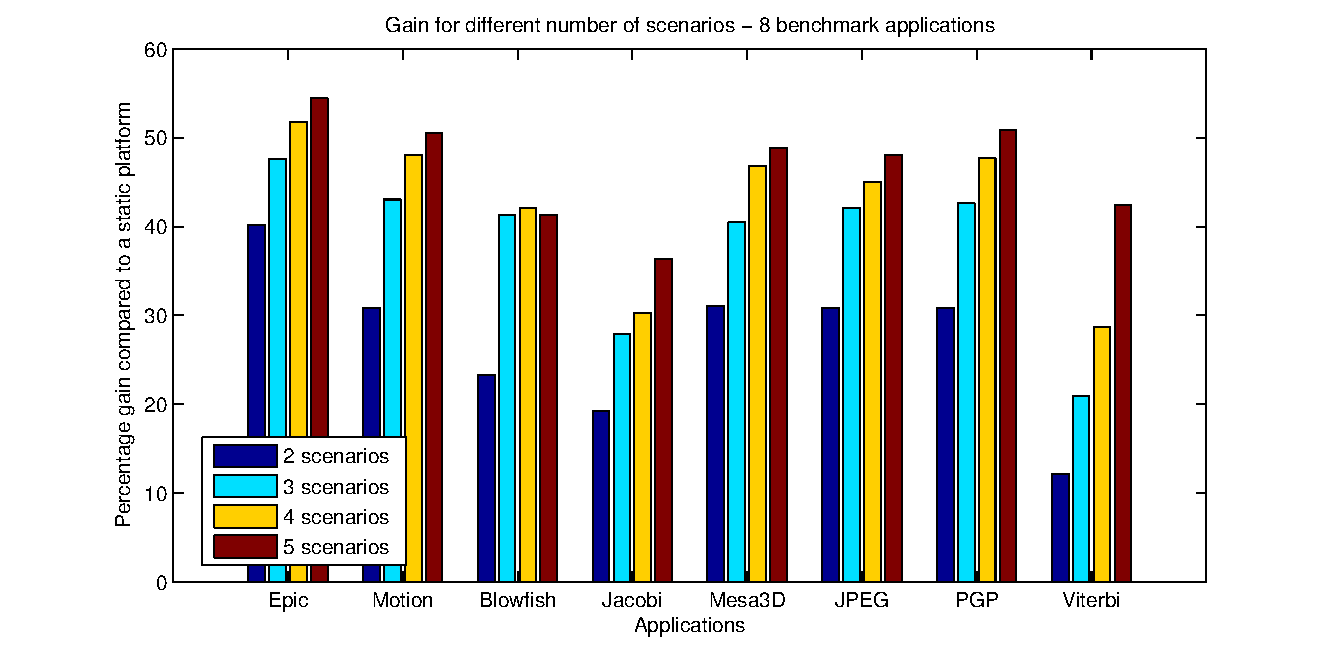
\includegraphics[width=\textwidth]{C/6appsGains.pdf}
\caption{Energy gain for increasing number of system scenarios - Static platform corresponds to 0\%}
\label{fig:gainsC}
\end{figure}

\begin{figure}
\centering
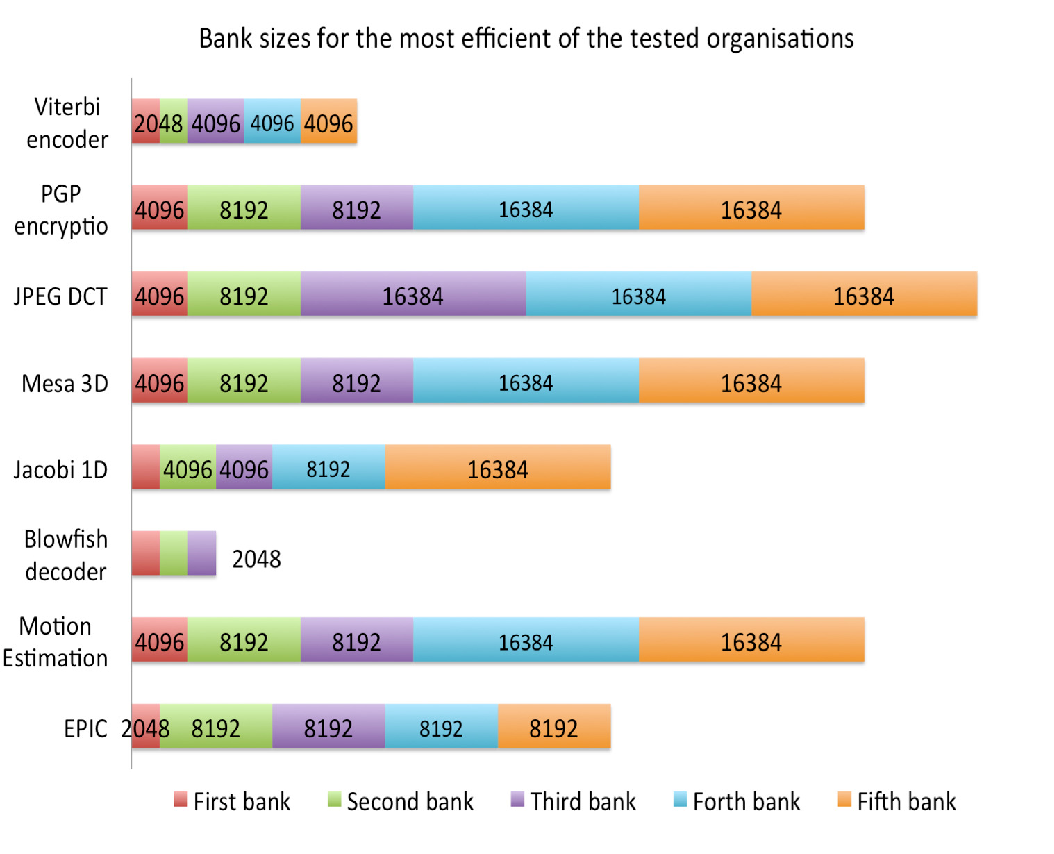
\includegraphics[width=0.75\textwidth]{C/banks2.pdf}
\caption{Bank sizes for the most efficient of the tested organisations for each benchmark}
\label{fig:banksC}
\end{figure}

\subsection{Classification of the Applications}

The introduction of a second system scenario results in energy gains between 15\% and  40\%  for the tested applications. 
Depending on the application's dynamism the maximum reported energy gains range from around 35\% to 55\%. 
As expected according to the categorisation presented in subsection~\ref{sec:categorisationC}, higher energy gains are achieved for applications with more dynamic memory requirements, i.e., bigger difference between the minimum and maximum allocated size. 
The maximum gains for JPEG, motion estimator, mesa 3D and PGP are around 50\% while blowfish, jacobi, and Viterbi decoders are around 40\%.

\begin{center}
	\begin{table}
	\caption{Range of energy gains on the memory subsystem}
	\label{tab:ranges}
	{
	\begin{tabular}{|c|c|c|c|c|c|c|c|}
		\hline
		\multicolumn{2}{|c|}{\textbf{EPIC}} &
		\multicolumn{2}{c|}{\textbf{Motion}} &
		\multicolumn{2}{c|}{\textbf{Blowfish}} &
		\multicolumn{2}{c|}{\textbf{Jacobi}}
		\\ 
		\cline{1-8}
		Min & Max & Min & Max & Min & Max & 
		Min & Max \\ 
		\hline 
		40.6\% & 55.1\% & 31.2\% & 50.1\% & 23.5\% & 42.0\% & 
		19.8\% & 35.9\% \\ 
		\hline 

		\multicolumn{2}{|c|}{\textbf{Mesa3D}} &
		\multicolumn{2}{c|}{\textbf{JPEG}} &
		\multicolumn{2}{c|}{\textbf{PGP}} &
		\multicolumn{2}{c|}{\textbf{Viterbi}} \\ 
		\cline{1-8}
		Min & Max & Min & Max & Min & Max & 
		Min & Max \\ 
		\hline 
		31.3\% & 49.2\% & 31.1\% & 48.9\% & 
		30.6\% & 51.2\% & 12.5\% & 42.4\% \\ 
		\hline
		
	\end{tabular}}
	\end{table}
\end{center}

As the number of system scenarios that are implemented on the memory subsystem increases, the energy gains improve since variations in memory requirements can be better exploited with more configurations. 
However, the improvement with increasing numbers of system scenarios differ depending on the kind of dynamism present in each application. 
The application with the highest variation in distribution of memory requirements is the Viterbi encoder/decoder and gains around 10\% is seen for every new memory bank added, even for a platform growing from four to five banks. 
In contrast, the application with the lowest number of different cases, blowfish, cannot further exploit a platform with more than three banks. 
Another case in which smaller energy gains are achieved, after a certain number of platform supported system scenarios have been reached, is the PGP encryption algorithm. 
In this benchmark the introduction of more scenarios has an energy impact of less than 5\% after the limit of three system scenarios has been reached. 

\subsection{Switching Overhead}

The switching cost increases for an increasing number of system scenarios due to the increasing frequency of platform reconfiguration. 
This overhead reduces the achieved gain, but for up to 5 scenarios we still see improvements for all but one of our benchmarks. 
The switching cost is below 2\% even for a platform with 5 memory banks in all cases.
Apart from the number of scenarios, the switching cost depends on the sensitivity of the variable used for scenario identification. 
A change of value on the identification variable indicates potentially a new scenario. 
For an increasing frequency of changes, the switching cost increases.

\subsection{Comparison with Use Case Scenario}

Comparative results from applying a use case scenario approach as a reference are presented in Fig.~\ref{fig:usecaseC}. 
Reported energy gains for both use case scenarios and the most efficient case of the system scenarios are given assuming a static platform as a base (0\%). 
Use case scenarios are generated based on a higher abstraction level that is visible as a user's behaviour. 
For example, use case scenarios for image processing applications generate three scenarios, if large, medium and small are the image sizes identified by the user. 
Similarly, use case scenarios for JPEG compression identify only low and high compression as options and motion estimation is performed on I, P and B video frames, without exploring fine grain differences inside a frame. 
In general, use case scenario identification can be seen as more coarse compared to identification on the detailed system implementation level. 
As seen in Fig.~\ref{fig:usecaseC} the use case gains are superior only to a static platform.

\begin{figure}
\centering
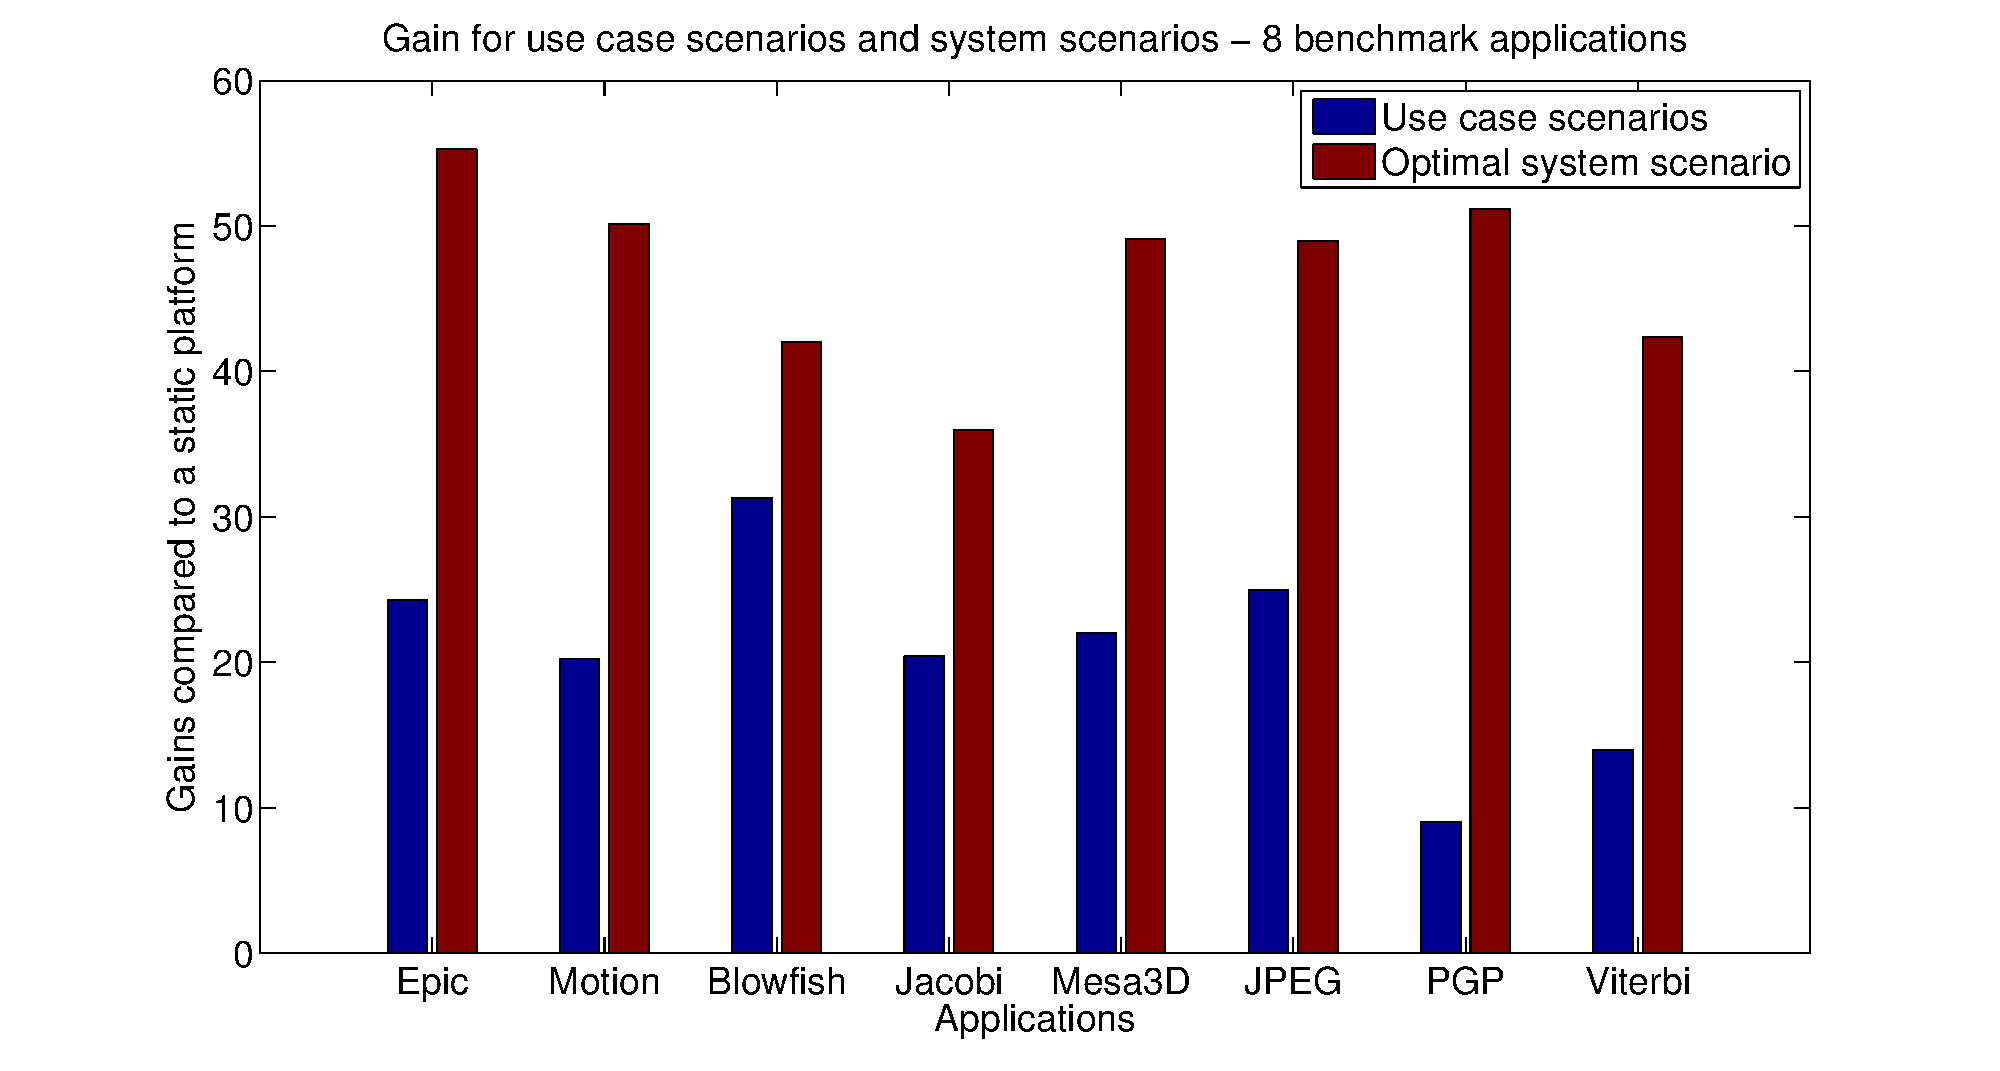
\includegraphics[width=\textwidth]{C/usecase.pdf}
\caption{Energy gain for use case scenarios and system scenarios}
\label{fig:usecaseC}
\end{figure}

\subsection{Run-Time Overhead}  

The reported energy gains are for the memory subsystem. 
As motivated in Section~\ref{sec:motivationC} this has previously been shown to be a major contributor to the total energy consumption. 
An additional energy overhead from the system scenario approach can be found in the processor performing the run-time system scenario detection and switching. 
This overhead is partly incorporated in $E_{SleepActive}$, in particular if traditional system scenarios are already implemented so that the only overhead is the addition of memory-awareness.
The run-time overhead is kept low, because the run-time manager is active for less than 1\% of the time needed for the execution of the application. 

\section{Conclusions}
\label{sec:conclusionC}

The scope of this work is to apply the memory-aware system scenario methodology to a wide range of multimedia application and test its effectiveness based on an extensive memory energy model. 
A wide range of applications is studied that allow us to draw conclusions about different kinds of dynamic behaviour and their effect on the energy gains achieved using the methodology. 
The results demonstrate the effectiveness of the methodology reducing the memory energy consumption with between 35\% and 55\%. 
Since memory size requirements are still met in all situations, performance is not reduced. 
The memory-aware system scenario methodology is suited for applications that experience dynamic behaviour with respect to memory organisation utilization during their execution.

\bibliographystyle{plain}
\bibliography{reference}
%\begin{thebibliography}{42}
%\providecommand{\natexlab}[1]{#1}
%\providecommand{\url}[1]{{#1}}
%\providecommand{\urlprefix}{URL }
%\expandafter\ifx\csname urlstyle\endcsname\relax
%  \providecommand{\doi}[1]{DOI~\discretionary{}{}{}#1}\else
%  \providecommand{\doi}{DOI~\discretionary{}{}{}\begingroup
%  \urlstyle{rm}\Url}\fi
%\providecommand{\eprint}[2][]{\url{#2}}
%
%\bibitem{Ben00b}
%Benini L, Macii A, Poncino M (2000) A recursive algorithm for
%  low-power memory partitioning. In: Proceedings of the 2000 intr symp on Low
%  Power Electronics and Design, pp 78 -- 83
%
%\bibitem{Ben00c}
%Benini L, et~al (2000) Increasing energy efficiency of embedded
%  systems by application-specific memory hierarchy generation. Design Test of
%  Computers, IEEE 17(2):74 --85, \doi{10.1109/54.844336}
%
%\bibitem{Gem5}
%Binkert N, et~al (2011) The gem5 simulator. SIGARCH Comput Archit News
%  39(2):1--7
%
%\bibitem{Che09}
%Cheung E, et~al (2009) Memory subsystem simulation in software tlm/t models.
%  In: Proceedings of Asia and South Pacific Design Automation Conference,
%  2009., pp 811 --816, \doi{10.1109/ASPDAC.2009.4796580}
%
%\bibitem{Chu02}
%Chung EY, et~al (2002) Contents provider-assisted dynamic voltage scaling for
%  low energy multimedia applications. In: Proceedings of the 2002 intr symp on
%  Low Power Electronics and Design, ISLPED '02, pp 42--47
%
%\bibitem{Fil12}
%Filippopoulos I, et~al (2012) Memory-aware system scenario approach energy
%  impact. In: NORCHIP, 2012, pp 1 --6, \doi{10.1109/NORCHP.2012.6403111}
%
%\bibitem{Garcia}
%Garcia P, et~al (2006) An overview of reconfigurable hardware in embedded
%  systems. EURASIP J Embedded Syst 2006(1):13--13
%
%\bibitem{Gheorghita2007}
%Gheorghita SV, et~al (2009) System-scenario-based design of dynamic embedded
%  systems. ACM Trans Des Autom Electron Syst 14(1):3:1--3:45
%
%\bibitem{Gonzalez1996}
%Gonzalez R, Horowitz M (1996) Energy dissipation in general purpose
%  microprocessors. Solid-State Circuits, IEEE Journal of 31(9):1277 --1284,
%  \doi{10.1109/4.535411}
%
%\bibitem{mibench}
%Guthaus M, Ringenberg J, Ernst D, Austin T, Mudge T, Brown R (2001) Mibench: A
%  free, commercially representative embedded benchmark suite. In: Workload
%  Characterization, 2001. WWC-4. 2001 IEEE Int. Workshop on, IEEE, pp 3--14
%
%\bibitem{Elena2010}
%Hammari E, Catthoor F, Kjeldsberg PG, Huisken J, (2010) Application of medium-grain multiprocessor mapping
%  methodology to epileptic seizure predictor. In: NORCHIP, 2010, pp 1 --6,
%  \doi{10.1109/NORCHIP.2010.5669489}
%  
%\bibitem{Elena2012}
%Hammari E, Catthoor F, Kjeldsberg PG, Huisken J, Tsakalis K, Iasemidis L, (2012) Realization of dynamical electronic systems. In: The International Conference on Engineering of Reconfigurable Systems and Algorithms, 2012 
%
%\bibitem{graybox}
%Himpe S, et~al (2002) {M}{T}{G}* and grey-box: modeling dynamic multimedia
%  applications with concurrency and non-determinism. In: System Specification
%  and Design Languages: Best of FDL02
%
%\bibitem{Hul11}
%Hulzink J, et~al (2011) An ultra low energy biomedical signal processing system
%  operating at near-threshold. IEEE Trans on Biomedical Circuits and Systems
%  5(6):546--554
%  
%\bibitem{Math}
%Ryser HJ (1963). Combinatorial mathematics. New York.
%
%\bibitem{Ang13b}
%Kritikakou A, et~al (2013) Near-optimal \& scalable intra-signal in-place for non-overlapping \& irregular access scheme. ACM Trans Design Automation of Electronic Systems (TODAES) ACM, New York, NY, USA.
%
%\bibitem{Ang13}
%Kritikakou A, et~al (2013) A scalable and near-optimal representation for storage size management. ACM Trans Architecture and Code Optimization. (accepted)
%
%\bibitem{mediabench}
%Lee C, et~al (1997) Mediabench: a tool for evaluating and synthesizing
%  multimedia and communicatons systems. In: Proceedings of the 30th annual
%  ACM/IEEE international symposium on Microarchitecture, IEEE Computer Society,
%  pp 330--335
%
%\bibitem{tcm}
%Ma Z, et~al (2007) Systematic Methodology for Real-Time Cost-Effective Mapping
%  of Dynamic Concurrent Task-Based Systems on Heterogenous Platforms, 1st edn.
%  Springer Publishing Company, Incorporated
%
%\bibitem{Mac02}
%Macii A, Benini L, Poncino M (2002) Memory Design Techniques for Low-Energy
%  Embedded Systems. Kluwer Academic Publishers
%
%\bibitem{Mar03}
%Marchal P, et~al (2003) {S}{D}{R}{A}{M} energy-aware memory allocation for
%  dynamic multi-media applications on multi-processor platforms. In: DATE, pp 516--521
%
%\bibitem{Mei10}
%Meinerzhagen P, Roth C, Burg A (2010) Towards generic low-power area-efficient
%  standard cell based memory architectures. In: Circuits and Systems (MWSCAS),
%  2010 53rd IEEE Int. Midwest Symposium on, IEEE, pp 129--132
%
%\bibitem{Mei11}
%Meinerzhagen P, et~al (2011) Benchmarking of standard-cell based memories in
%  the sub-vt domain in 65-nm cmos technology. IEEE Transactions on Emerging and
%  Selected Topics in Circuits and Systems 1(2)
%
%\bibitem{narasinga}
%Miniskar NR (2012) System scenario based resource management of processing
%  elements on mpsoc. PhD thesis, Katholieke Universiteit Leuven
%
%\bibitem{Pal06}
%Palkovic M, Catthoor F, Corporaal H (2006) Dealing with variable
%  trip count loops in system level exploration. In: Proceedings of the 4th Workshop
%  on Optimizations for DSP and Embedded Systems, IEEE and ACM SIGMICRO, pp
%  21--30
%
%\bibitem{Pal07}
%Palkovic M, Corporaal H, Catthoor F (2007) Heuristics for scenario creation to
%  enable general loop transformations. In: System-on-Chip, 2007 Int. Symposium
%  on, pp 1 --4
%\bibitem{Pal06b}
%Palkovic M, et~al (2006) Systematic preprocessing of data
%  dependent constructs for embedded systems. Journal of Low Power Electronics,
%  Volume 2, Number 1
%
%\bibitem{Pgk01}
%Panda PR, et~al (2001) Data and memory optimization techniques for embedded
%  systems. ACM Trans Des Autom Electron Syst 6(2):149--206
%
%\bibitem{Poly}
%Pouchet L (2012) Polybench: The polyhedral benchmark suite
%
%\bibitem{Ben99}
%Simunic T, et~al (1999) Cycle-accurate simulation of energy consumption in
%  embedded systems. In: Proceedings of the 36th Design Automation Conference,
%  1999., pp 867--872
%  
%\bibitem{abraham1999automatic}
%Abraham SG, Mahlke SA (1999) Automatic and efficient evaluation of memory
%  hierarchies for embedded systems. In: Proceedings of the Microarchitecture, 1999. MICRO-32.
%  . 32nd Annual International Symposium on, IEEE, pp 114--125
%
%\bibitem{chen1999loop}
%Chen F, Sha EHM (1999) Loop scheduling and partitions for hiding memory
%  latencies. In: Proceedings of the 12th international symposium on System
%  synthesis, IEEE Computer Society, p~64
%
%\bibitem{chen2000synthesis}
%Chen S, Postula A (2000) Synthesis of custom interleaved memory systems. Very
%  Large Scale Integration (VLSI) Systems, IEEE Transactions on 8(1):74--83
%
%\bibitem{grun2000mist}
%Grun P, Dutt N, Nicolau A (2000) Mist: An algorithm for memory miss traffic
%  management. In: Proceedings of the 2000 IEEE/ACM international conference on
%  Computer-aided design, IEEE Press, pp 431--438
%
%\bibitem{jacob1996analytical}
%Jacob BL, Chen PM, Silverman SR, Mudge TN (1996) An analytical model for
%  designing memory hierarchies. Computers, IEEE Transactions on
%  45(10):1180--1194
%
%\bibitem{jantsch1994hardware}
%Jantsch A, Ellervee P, Hemani A, {\"O}berg J, Tenhunen H (1994)
%  Hardware/software partitioning and minimizing memory interface traffic. In:
%  Proceedings of the conference on European design automation, IEEE Computer
%  Society Press, pp 226--231
%
%\bibitem{kandemir2001improving}
%Kandemir M, Sezer U, Delaluz V (2001) Improving memory energy using access
%  pattern classification. In: Proceedings of the 2001 IEEE/ACM international
%  conference on Computer-aided design, IEEE Press, pp 201--206
%
%\bibitem{li1999hardware}
%Li Y, Wolf WH (1999) Hardware/software co-synthesis with memory hierarchies.
%  In: Computer-Aided Design of Integrated Circuits and Systems, IEEE Transactions
%  on 18(10):1405--1417
%
%\bibitem{oshima1997high}
%Oshima Y, Sheu BJ, Jen SH (1997) High-speed memory architectures for multimedia
%  applications. Circuits and Devices Magazine, IEEE 13(1):8--13
%
%\bibitem{passes1995multi}
%Passes N, Sha EM, Chao LF (1995) Multi-dimensional interleaving for
%  time-and-memory design optimization. In: Proceedings of the Computer Design: VLSI in Computers
%  and Processors, 1995. ICCD'95, 1995 IEEE International
%  Conference on, IEEE, pp 440--445
%
%\bibitem{schmit1997synthesis}
%Schmit H, Thomas DE (1997) Synthesis of application-specific memory designs.
%  Very Large Scale Integration (VLSI) Systems, IEEE Transactions on
%  5(1):101--111
% 
%\bibitem{usecase}
%Gutierrez JJ, et~al (2008). A case study for generating test cases from use cases. In: Research Challenges in Information Science, 2008. RCIS 2008. Second International Conference on (pp. 209-214). IEEE.
%
%\end{thebibliography}
%
%
%\end{document}
